\chapter{Identifying Substances}\label{ch:g7:identifying-substances}

A crumpled note, written in black felt-tip, is found at the scene of a
small mystery, and three felt-tip pens are found in three different
bags. To the eye the three inks look the same black. A forensic chemist
needs only a strip of paper, a little water and half an hour to say
which pen wrote the note. Chemists identify substances not by how they
look, but by how they behave in a test chosen for them.

\begin{recall}
A \omterm{def:g6:pure-substances-and-mixtures:species}{chemical species} is one particular kind of substance; a \omterm{def:g6:pure-substances-and-mixtures:pure-substance}{pure substance}
holds one single species, a \omterm{def:g6:pure-substances-and-mixtures:mixture}{mixture} several
(\cref{ch:g6:pure-substances-and-mixtures}). Some substances \omterm{def:g2:mixing-and-dissolving:dissolve}{dissolve}
well in a \omterm{def:g6:solutions-and-solubility:solute}{solvent}, others little or not at all: each has its own
\omterm{def:g6:solutions-and-solubility:solubility}{solubility} (\cref{ch:g6:solutions-and-solubility}).
\end{recall}

\section{What a characteristic test is}

\begin{definition}[Characteristic test and reagent]\label{def:g7:identifying-substances:characteristic-test}
A \emph{characteristic test}\index{characteristic test} for a \omterm{def:g6:pure-substances-and-mixtures:species}{chemical
species} is a simple experiment that gives a visible result with that
species, and not with the others met in the same situation. It uses a
substance chosen for the purpose, the
\emph{reagent}\index{reagent}.
\end{definition}


\begin{method}[Running a characteristic test]\label{met:g7:identifying-substances:run}
\begin{enumerate}
  \item Take a small sample of the substance to be tested.
  \item Add the \omterm{def:g7:identifying-substances:characteristic-test}{reagent}, or bring it into contact with the sample, as
        the test describes.
  \item Observe: a colour change, a cloudiness, a flame, a sound.
  \item Conclude: the test is \emph{positive} if the expected result
        appears, \emph{negative} if it does not.
  \item Run the same test on a sample known not to contain the species
        (a blank): it must stay negative, otherwise the result proves
        nothing.
\end{enumerate}
\end{method}

\section{Four classic tests}

\begin{proposition}[Carbon dioxide turns limewater milky]\label{prop:g7:identifying-substances:limewater}
Limewater is a clear, colourless solution. When carbon dioxide is
bubbled through it, it turns milky, cloudy white. \omterm{def:g4:air-a-mixture-of-gases:air}{Air} breathed out
through a straw turns limewater milky; fresh \omterm{def:g4:air-a-mixture-of-gases:air}{air} pumped through it
hardly does.
\end{proposition}

\begin{omfigure}
\begin{tikzpicture}[font=\small, scale=1.25]
  % generating tube, stoppered
  \pic[transform shape] at (0,0) {testtube={0.35}{omWater!80}};
  \fill[black!65] (-0.27,2.8) rectangle (0.27,3.15);
  \foreach \y in {0.4,0.65,0.85} \draw[black!55] (0.05,\y) circle (0.04);
  \pic[transform shape] at (0,2.9) {deliverytube={1.9}{-2.3}};
  % limewater tube
  \pic[transform shape] at (1.9,0) {testtube={0.6}{white!85!black}};
  \foreach \x/\y in {1.88/0.75,1.95/1.0,1.85/1.25,1.92/1.5} \draw[black!55] (\x,\y) circle (0.04);
  \draw[<-, omProp, thick] (-0.3,0.5) -- (-1.2,0.8) node[left, text=black, align=right]
    {a reaction\\ giving off a gas};
  \draw[<-, omProp, thick] (2.2,1.2) -- (3.0,1.4) node[right, text=black, align=left]
    {limewater turns\\ milky: the gas is\\ carbon dioxide};
\end{tikzpicture}

{\small The limewater test. The gas given off in the first tube bubbles
through limewater; if the limewater turns milky, the gas is carbon
dioxide.}
\end{omfigure}

\begin{proposition}[Water turns anhydrous copper sulfate blue]\label{prop:g7:identifying-substances:copper-sulfate}
Anhydrous copper sulfate is a white powder. A drop of water turns it
blue at once. The test shows that water is present, in a liquid or in a
damp solid --- not that the liquid is pure water.
\end{proposition}

\begin{omfigure}
\begin{minipage}[b]{0.48\linewidth}\centering
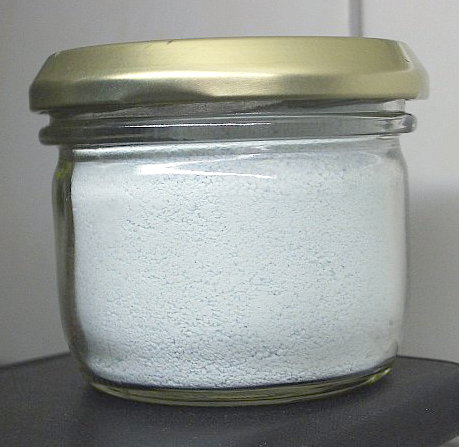
\includegraphics[width=\linewidth,height=4.2cm,keepaspectratio]{images/book1/cuso4-anhydrous.jpg}

{\small Anhydrous copper sulfate: a white powder. Photo: W.~Oelen,
CC BY-SA 3.0.}
\end{minipage}\hfill
\begin{minipage}[b]{0.48\linewidth}\centering
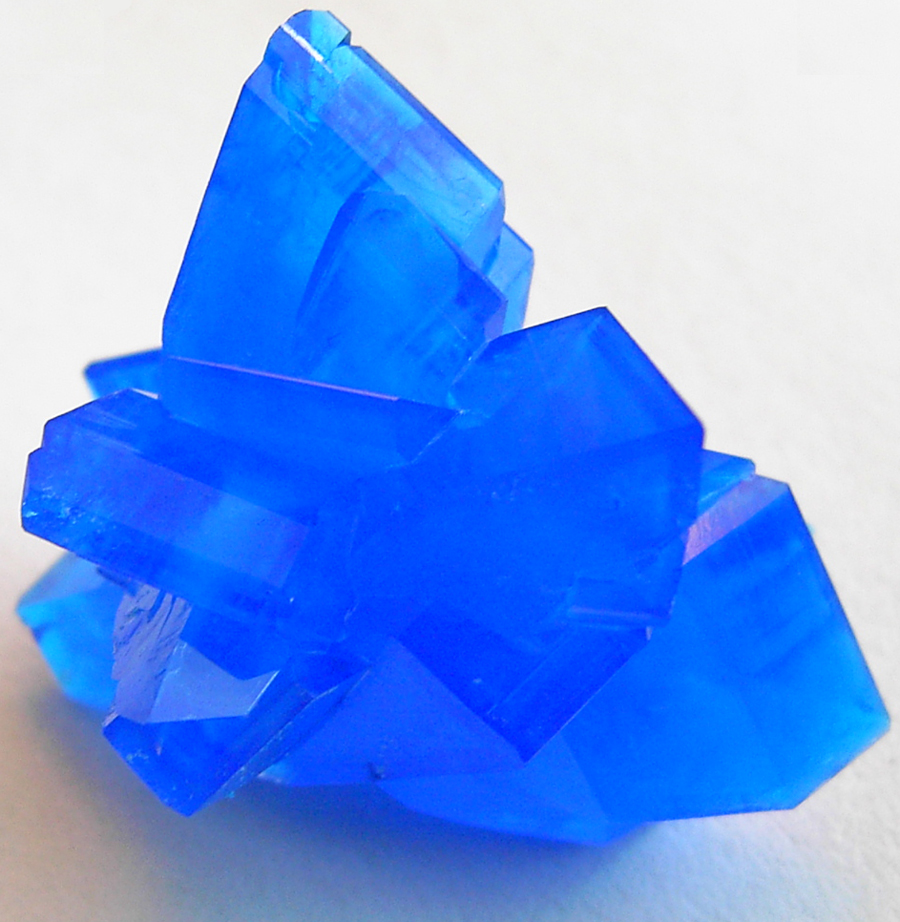
\includegraphics[width=\linewidth,height=4.2cm,keepaspectratio]{images/book1/cuso4-hydrated.jpg}

{\small With water it turns blue; these crystals hold water. Photo:
Stephanb, CC BY-SA 3.0.}
\end{minipage}
\end{omfigure}

\begin{safety}{\ghs[0.82cm]{GHS05}\ghs[0.82cm]{GHS07}\ghs[0.82cm]{GHS09}}
% ledger: ghs:CuSO4
Copper sulfate: harmful if swallowed and irritating to the skin (GHS07);
it can seriously damage the eyes (GHS05); very toxic to aquatic life,
with long-lasting effects (GHS09). Goggles and gloves; the waste is
collected, never poured down the sink.
\end{safety}

\begin{proposition}[Oxygen relights a glowing splint]\label{prop:g7:identifying-substances:splint}
A wooden splint is lit, then blown out so that only a red glow remains.
Pushed into a test tube of oxygen, the glowing splint bursts back into
flame.
\end{proposition}

\begin{proposition}[Hydrogen burns with a squeaky pop]\label{prop:g7:identifying-substances:pop}
A lighted splint held at the mouth of a small test tube of hydrogen
makes a short, squeaky ``pop'': the hydrogen burns at once with the
oxygen of the \omterm{def:g4:air-a-mixture-of-gases:air}{air}.
\end{proposition}

\begin{omfigure}
\begin{tikzpicture}[font=\small, scale=1.25]
  % splint test for oxygen
  \pic[transform shape] at (0,0) {testtube={0}{white}};
  \draw[brown!60!black, line width=2pt] (0.15,1.6) -- (1.4,3.6);
  \fill[orange!85] (0.15,1.6) circle (0.07);
  \fill[orange!80] (0.12,1.62) .. controls (0.0,1.9) and (0.08,2.1) .. (0.1,2.3)
    .. controls (0.2,2.05) and (0.3,1.85) .. (0.2,1.62);
  \node[anchor=north, align=center] at (0,-0.15) {oxygen:\\ the glowing splint\\ bursts into flame};
  % pop test for hydrogen
  \begin{scope}[xshift=4cm]
    \pic[transform shape, rotate=180] at (0,3.1) {testtube={0}{white}};
    \draw[brown!60!black, line width=2pt] (0.05,-0.05) -- (1.3,-0.9);
    \fill[orange!85] (0.05,-0.02) .. controls (-0.05,0.08) and (0.0,0.15) .. (0.02,0.22)
      .. controls (0.08,0.15) and (0.15,0.08) .. (0.1,-0.02);
    \node[font=\small\itshape] at (-0.9,0.15) {pop!};
    \node[anchor=north, align=center] at (0,-1.0) {hydrogen:\\ a squeaky pop\\ at the mouth};
  \end{scope}
\end{tikzpicture}

{\small Left: a glowing splint relights in oxygen. Right: a lighted
splint at the mouth of an upturned tube of hydrogen gives a squeaky pop
(hydrogen is lighter than \omterm{def:g4:air-a-mixture-of-gases:air}{air}, so the tube is held mouth down).}
\end{omfigure}

\begin{safety}{\ghs[0.82cm]{GHS02}\ghs[0.82cm]{GHS04}}
% ledger: ghs:H2
Hydrogen: extremely flammable gas (GHS02), stored under pressure in
cylinders (GHS04). The pop test is made with a few millilitres only, by
the teacher.
\end{safety}

\section{Paper chromatography}

\begin{definition}[Paper chromatography and chromatogram]\label{def:g7:identifying-substances:chromatography}
\emph{Paper chromatography}\index{paper chromatography} separates the
dyes of a \omterm{def:g6:pure-substances-and-mixtures:mixture}{mixture}. A small spot of the \omterm{def:g6:pure-substances-and-mixtures:mixture}{mixture} is put on a line drawn
near the bottom of a strip of paper; the bottom of the strip dips into a
\omterm{def:g6:solutions-and-solubility:solute}{solvent}, which slowly climbs up the paper and carries each dye with it,
some faster than others. When the \omterm{def:g6:solutions-and-solubility:solute}{solvent} has climbed almost to the top,
the strip is taken out and dried: it is the
\emph{chromatogram}\index{chromatogram}.
\end{definition}

\begin{omfigure}
\begin{tikzpicture}[font=\small, scale=1.3]
  % the strip in a beaker of solvent
  \pic[transform shape] at (0,0) {beaker={0.12}{omWater!80}};
  \fill[white] (-0.42,0.06) rectangle (0.42,2.2);
  \fill[omWater!80] (-0.42,0.06) rectangle (0.42,0.24);
  \draw[omGlass, line width=0.6pt] (-0.42,0.06) rectangle (0.42,2.2);
  \draw[black!60, line width=0.4pt] (-0.42,0.42) -- (0.42,0.42);
  \fill[black!80] (0,0.42) circle (0.07);
  \shade[ball color=black!20] (0,2.27) circle (0.08);
  \draw[black!50, line width=1.2pt] (-1.1,2.27) -- (1.1,2.27);
  \node[anchor=north, align=center] at (0,-0.15) {at the start};
  \draw[<-, omProp, thick] (0.1,0.5) -- (1.3,0.8) node[right, text=black]
    {ink spot on a pencil line};
  \draw[<-, omProp, thick] (1.0,2.27) -- (1.3,2.5) node[right, text=black]
    {glass rod holding the paper};
  \draw[<-, omProp, thick] (0.75,0.15) -- (1.3,0.25) node[right, text=black]
    {solvent, below the line};
  % the chromatogram
  \begin{scope}[xshift=6.2cm]
    \pic[transform shape] at (0,0) {tlcplate};
    \draw[black!50, dashed] (-0.7,2.7) -- (0.7,2.7);
    \fill[blue!70] (0,1.0) ellipse (0.13 and 0.09);
    \fill[red!70] (0,1.7) ellipse (0.13 and 0.09);
    \fill[yellow!80!orange] (0,2.35) ellipse (0.13 and 0.09);
    \node[anchor=north, align=center] at (0,-0.15) {the chromatogram};
    \draw[<-, omProp, thick] (0.75,2.7) -- (1.3,2.85) node[right, text=black]
      {how far the solvent climbed};
    \draw[<-, omProp, thick] (0.2,1.7) -- (1.3,1.7) node[right, text=black]
      {three dyes: the ink is a mixture};
  \end{scope}
\end{tikzpicture}

{\small \omterm{def:g7:identifying-substances:chromatography}{Paper chromatography} of a black ink. The \omterm{def:g6:solutions-and-solubility:solute}{solvent} rises through
the paper and separates the ink into three dyes.}
\end{omfigure}

\begin{method}[Reading a chromatogram]\label{met:g7:identifying-substances:read}
\begin{enumerate}
  \item Count the spots above each starting point: one spot, one dye; two
        spots or more, a \omterm{def:g6:pure-substances-and-mixtures:mixture}{mixture} of dyes.
  \item Compare heights: in the same \omterm{def:g7:identifying-substances:chromatography}{chromatogram}, one dye always climbs
        to the same height. A spot at the same height as a known dye is
        probably that dye.
  \item Use a pencil line, never ink: ink would itself be separated by
        the \omterm{def:g6:solutions-and-solubility:solute}{solvent}.
\end{enumerate}
\end{method}

\begin{example}[The dyes of sweets]\label{ex:g7:identifying-substances:sweets}
The coloured coatings of sweets are scraped into a little water and
spotted on a strip, beside spots of the food dyes allowed in sweets.
The \omterm{def:g7:identifying-substances:chromatography}{chromatogram} shows that the green coating holds a yellow dye and a
blue dye, both found among the allowed dyes.
\end{example}


\section{Reading a test bank}

\begin{proposition}[A table of characteristic tests]\label{prop:g7:identifying-substances:bank}
Chemists keep the tests they use in a table, a test bank, which reads
from left to right:
\begin{center}
\small
\begin{tabular}{llll}
\hline
species looked for & \omterm{def:g7:identifying-substances:characteristic-test}{reagent} or test & positive result & \\
\hline
carbon dioxide & limewater & limewater turns milky & \\
water & anhydrous copper sulfate & white turns blue & \\
oxygen & glowing splint & the splint relights & \\
hydrogen & lighted splint & a squeaky pop & \\
dyes of a \omterm{def:g6:pure-substances-and-mixtures:mixture}{mixture} & \omterm{def:g7:identifying-substances:chromatography}{paper chromatography} & one spot per dye & \\
\hline
\end{tabular}
\end{center}
\end{proposition}

\begin{remark}[What a test does not say]\label{rem:g7:identifying-substances:limits}
A positive test proves that the species is present, not that it is
alone: a liquid that turns copper sulfate blue contains water, but it
may be salty water or orange juice. A negative test only says that the
species is absent, or present in too small an amount to show.
\end{remark}

\begin{omfigure}
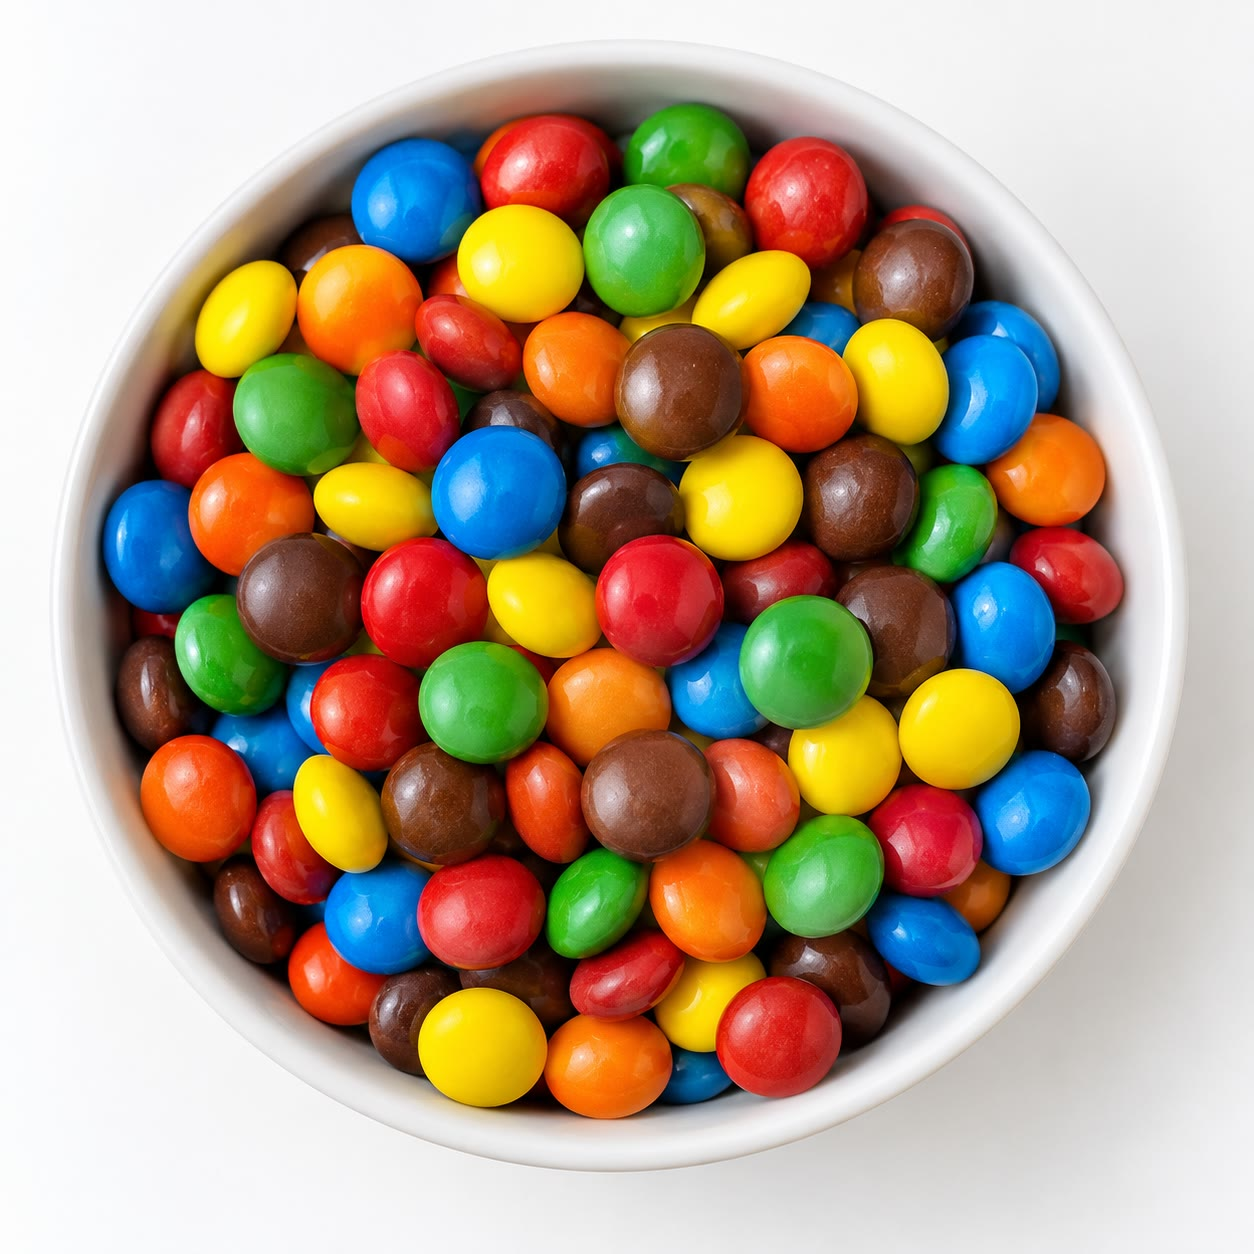
\includegraphics[width=0.32\linewidth]{images/book1/ai/g7-sweets.jpg}

{\small Sugar-coated sweets: their colours are \omterm{def:g6:pure-substances-and-mixtures:mixture}{mixtures} of dyes that
chromatography can separate.}
\end{omfigure}

\begin{omfigure}
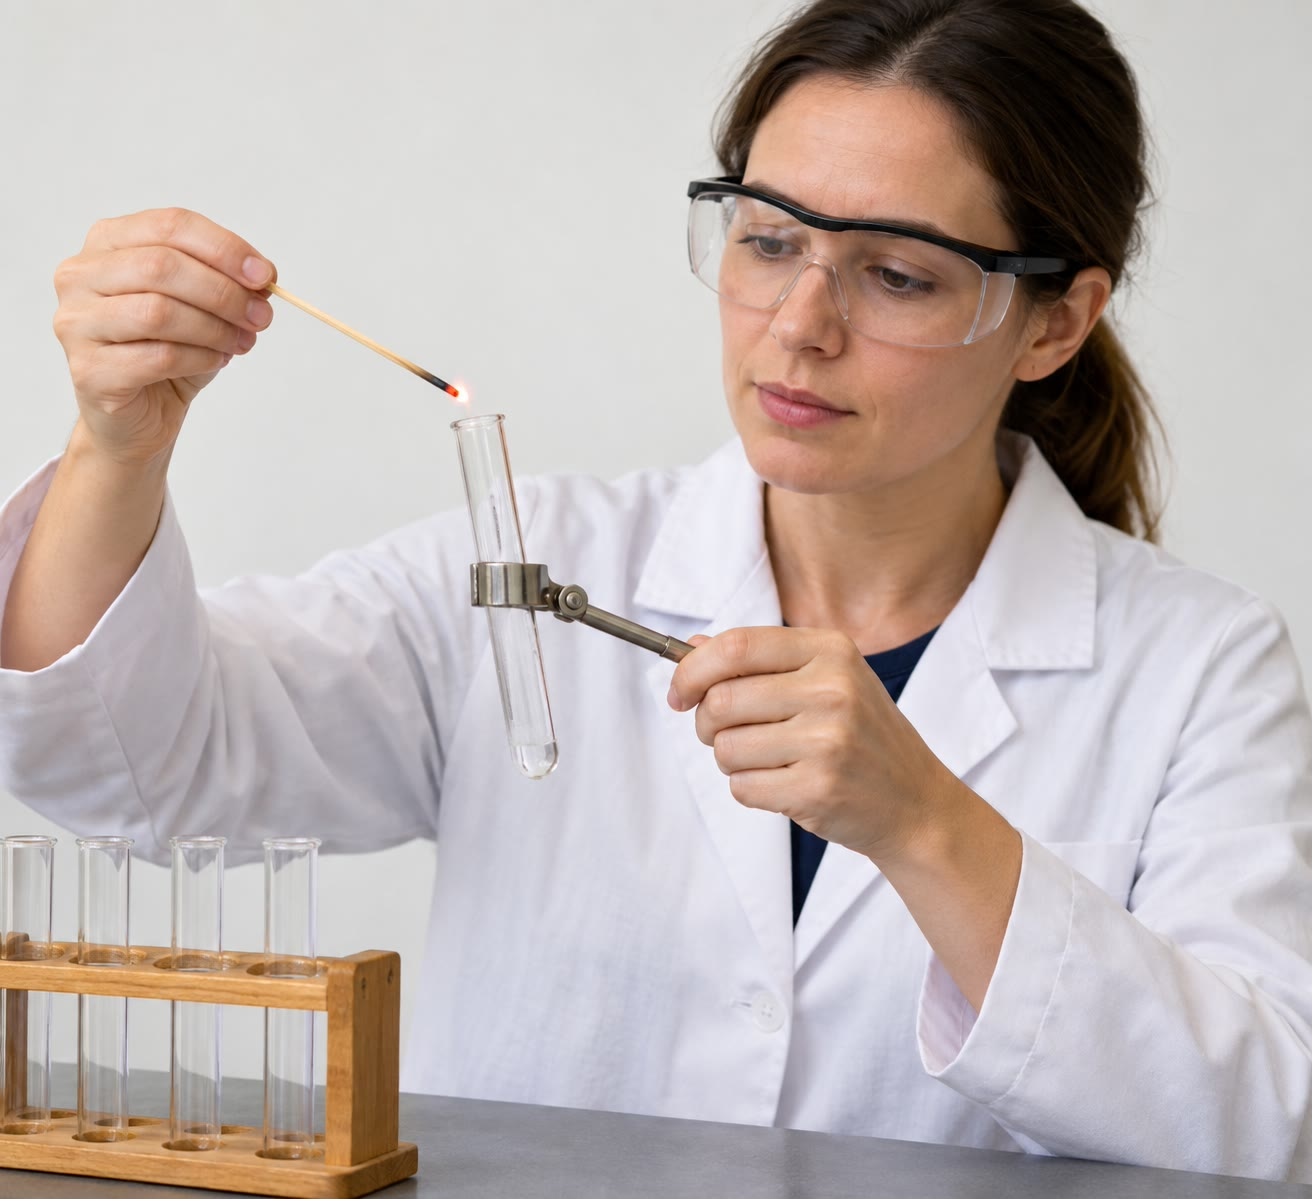
\includegraphics[width=0.36\linewidth]{images/book1/ai/g7-splint-teacher.jpg}

{\small A teacher tests a gas with a glowing splint.}
\end{omfigure}

\section{Exercises}

\begin{exercise}[$\star$]\label{exo:g7:identifying-substances:1}
Which test identifies carbon dioxide? Describe its positive result.
\end{exercise}

\begin{exercise}[$\star$]\label{exo:g7:identifying-substances:2}
A white powder turns blue when a liquid is dropped on it. What does
this show about the liquid?
\end{exercise}

\begin{exercise}[$\star$]\label{exo:g7:identifying-substances:3}
A glowing splint is put into a gas jar and bursts into flame. Which gas
does the jar hold?
\end{exercise}

\begin{exercise}[$\star$]\label{exo:g7:identifying-substances:4}
Why is the starting line of a paper \omterm{def:g7:identifying-substances:chromatography}{chromatogram} drawn in pencil and
not in ink?
\end{exercise}

\begin{exercise}[$\star\star$]\label{exo:g7:identifying-substances:5}
Why must the starting line be above the level of the \omterm{def:g6:solutions-and-solubility:solute}{solvent} in the
beaker?
\end{exercise}

\begin{exercise}[$\star\star$]\label{exo:g7:identifying-substances:6}
A \omterm{def:g7:identifying-substances:chromatography}{chromatogram} of a green ink shows two spots, one at the height of a
yellow reference dye, one at the height of a blue reference dye. Is the
green ink a \omterm{def:g6:pure-substances-and-mixtures:pure-substance}{pure substance}? What is it made of?
\end{exercise}

\begin{exercise}[$\star\star$]\label{exo:g7:identifying-substances:7}
Using the test bank, which test would you use to show that a gas given
off by a reaction is hydrogen? What do you expect to see?
\end{exercise}

\begin{exercise}[$\star\star$]\label{exo:g7:identifying-substances:8}
\omterm{def:g4:air-a-mixture-of-gases:air}{Air} breathed out turns limewater milky much faster than fresh \omterm{def:g4:air-a-mixture-of-gases:air}{air}.
What does this tell us about the \omterm{def:g4:air-a-mixture-of-gases:air}{air} we breathe out?
\end{exercise}

\begin{exercise}[$\star\star$]\label{exo:g7:identifying-substances:9}
A clear liquid turns anhydrous copper sulfate blue. Sam concludes:
``It is pure water.'' Explain why Sam is wrong.
\end{exercise}

\begin{exercise}[$\star\star$]\label{exo:g7:identifying-substances:10}
Look at the \omterm{def:g7:identifying-substances:chromatography}{chromatogram} of the black ink in this chapter. How many dyes
does the ink contain? Which one climbed highest?
\end{exercise}

\begin{exercise}[$\star\star\star$]\label{exo:g7:identifying-substances:11}
Three jars hold oxygen, hydrogen and carbon dioxide, but their labels are
lost. Plan, on paper, the tests that would name each jar, in an order
that uses as few tests as possible.
\end{exercise}

\begin{exercise}[$\star\star\star$]\label{exo:g7:identifying-substances:12}
A student tests a gas with limewater and sees nothing happen. Give two
possible explanations, and the control test that would help decide.
\end{exercise}

\section{Problem: The Forged Note}

\begin{problem}[{Weekend problem --- a felt-tip note, three suspect pens,
three unlabelled gas cylinders, and a test bank}]
\label{pb:g7:identifying-substances:1}
A school laboratory is asked to help with two small mysteries. First, a
note written in black felt-tip must be matched to one of three black
pens, 1, 2 and 3. A drop of ink is taken from the note and from each pen
and spotted on the same strip of paper, which is then developed with
water. The \omterm{def:g7:identifying-substances:chromatography}{chromatogram} is shown below.
\begin{center}
\begin{tikzpicture}[font=\small, x=1cm, y=1cm]
  \fill[white] (0,0) rectangle (6,4);
  \draw[omGlass, line width=0.6pt] (0,0) rectangle (6,4);
  \draw[black!60] (0,0.5) -- (6,0.5);
  \draw[black!50, dashed] (0,3.6) -- (6,3.6);
  \foreach \x/\lab in {0.9/note, 2.3/pen 1, 3.7/pen 2, 5.1/pen 3}
    \node[anchor=north] at (\x,-0.05) {\lab};
  % note: three dyes
  \fill[blue!70] (0.9,1.2) ellipse (0.18 and 0.1);
  \fill[red!70] (0.9,2.2) ellipse (0.18 and 0.1);
  \fill[yellow!80!orange] (0.9,3.1) ellipse (0.18 and 0.1);
  % pen 1: two dyes
  \fill[blue!70] (2.3,1.2) ellipse (0.18 and 0.1);
  \fill[black!70] (2.3,2.7) ellipse (0.18 and 0.1);
  % pen 2: same three as the note
  \fill[blue!70] (3.7,1.2) ellipse (0.18 and 0.1);
  \fill[red!70] (3.7,2.2) ellipse (0.18 and 0.1);
  \fill[yellow!80!orange] (3.7,3.1) ellipse (0.18 and 0.1);
  % pen 3: three dyes, other heights
  \fill[violet!70] (5.1,0.9) ellipse (0.18 and 0.1);
  \fill[red!70] (5.1,1.8) ellipse (0.18 and 0.1);
  \fill[green!60!black] (5.1,2.6) ellipse (0.18 and 0.1);
  \node[anchor=west, font=\footnotesize] at (6.1,3.6) {solvent front};
  \node[anchor=west, font=\footnotesize] at (6.1,0.5) {starting line};
\end{tikzpicture}
\end{center}

\medskip
\noindent\textbf{Part I --- The \omterm{def:g7:identifying-substances:chromatography}{chromatogram}.}
\begin{enumerate}
  \item Why were all four inks spotted on the same strip and developed
        together?
  \item Is the ink of the note a \omterm{def:g6:pure-substances-and-mixtures:pure-substance}{pure substance} or a \omterm{def:g6:pure-substances-and-mixtures:mixture}{mixture}? Explain.
  \item How many dyes does the ink of pen 1 contain? Can pen 1 have
        written the note?
  \item Pen 3 also contains three dyes. Why can it not have written the
        note?
  \item Which pen matches the note? Explain using the heights of the
        spots.
\end{enumerate}

\medskip
\noindent\textbf{Part II --- Three gas cylinders.}
The second mystery: three small cylinders, X, Y and Z, have lost their
labels; they hold oxygen, hydrogen and carbon dioxide. A little gas from
each is collected in a test tube. Gas X relights a glowing splint. Gas Y
makes a squeaky pop with a lighted splint. Gas Z turns limewater milky.
\begin{enumerate}[resume]
  \item Name gas X.
  \item Name gas Y.
  \item Name gas Z.
  \item Before testing gas Z, the student bubbles ordinary \omterm{def:g4:air-a-mixture-of-gases:air}{air} through
        the same limewater for the same time, and it stays clear. What is
        this second test called, and what does it add to the conclusion?
\end{enumerate}

\medskip
\noindent\textbf{Part III --- The test bank.}
\begin{enumerate}[resume]
  \item A colourless liquid found next to the note turns anhydrous
        copper sulfate blue. Write the line of the test bank used, and
        what the result shows.
  \item Does this result prove that the liquid is pure water? Explain.
  \item Conclude the first mystery: how many dyes does the ink of the
        note contain, and which pen wrote it?
\end{enumerate}
\end{problem}
